%%%%%%%%%%%%%%%%%%%%%%%%%%%%%%%%%%%%%%%%%
% University/School Laboratory Report
% LaTeX Template
% Version 3.1 (25/3/14)
%
% This template has been downloaded from:
% http://www.LaTeXTemplates.com
%
% Original author:
% Linux and Unix Users Group at Virginia Tech Wiki 
% (https://vtluug.org/wiki/Example_LaTeX_chem_lab_report)
%
% License:
% CC BY-NC-SA 3.0 (http://creativecommons.org/licenses/by-nc-sa/3.0/)
%
%%%%%%%%%%%%%%%%%%%%%%%%%%%%%%%%%%%%%%%%%

%----------------------------------------------------------------------------------------
%	PACKAGES AND DOCUMENT CONFIGURATIONS
%----------------------------------------------------------------------------------------

\documentclass{article}
\usepackage[spanish,es-tabla]{babel}

\usepackage[a4paper,
 %left=20mm,
 top=30mm,
 bottom=25mm,
 headheight=80pt,
 headsep=15mm
 ]{geometry}


\usepackage[version=3]{mhchem} % Package for chemical equation typesetting
\usepackage{graphicx} % Required for the inclusion of images

\usepackage{amsfonts}
\usepackage{amsmath} % Required for some math elements 
\usepackage{mathtools}
\DeclarePairedDelimiter{\ceil}{\lceil}{\rceil} %this is for ceil and floor symbols
\DeclarePairedDelimiter{\floor}{\lfloor}{\rfloor} %this is for ceil and floor symbols

\usepackage{changepage} % Required in text margins
\usepackage{xcolor} % Required changing color 
\usepackage{sectsty} %Required to change section headers
\usepackage{titlesec} % Required for section spacing
\usepackage{enumitem}
\usepackage{tocloft} % Better in table of contents
\usepackage[blocks]{authblk}% The option is for block layout
\usepackage[pdfborder={0 0 0}]{hyperref}% For email addresses
\usepackage{fancyhdr} %Required for Headers

\usepackage[nottoc]{tocbibind} %Better to add references and more in table of contents (nottoc is to remove indice in toc)

\usepackage{layout} %Used for "margin debugging"

\usepackage[export]{adjustbox} 
\usepackage{subcaption}

\pagestyle{fancy}
\fancyheadoffset{0cm} %Used for heading without margins
\fancyhead[L]{} % 1. sectionname

\rhead{Simulaci\'on y Animaci\'on Biomec\'anica de un Humanoide}
\renewcommand{\headrulewidth}{0.4pt}


\renewcommand\cfttoctitlefont{\hfill\huge\bfseries\color{cyan}}
\renewcommand\cftaftertoctitle{\hfill\mbox{}}

\setlist{leftmargin=5.5mm}

\titlespacing*{\section} {0pt}{6ex}{2ex}
\titlespacing*{\subsection} {0pt}{4ex}{0.7ex}

\sectionfont{\color{cyan}} % Changing color to section headers
\subsectionfont{\color{cyan}} % Changing color to subsection headers
\subsubsectionfont{\color{cyan}} % Changing color to subsubsection headers

%\setlength\parindent{0pt} % Removes all indentation from paragraphs

\renewcommand{\labelitemi}{$-$}

\renewcommand{\baselinestretch}{1.25} 

\renewcommand{\labelenumi}{\alph{enumi}.} % Make numbering in the enumerate environment by letter rather than number (e.g. section 6)

%\usepackage{times} % Uncomment to use the Times New Roman font

%----------------------------------------------------------------------------------------
%	DOCUMENT INFORMATION
%----------------------------------------------------------------------------------------

\title{\textbf{\\PROYECTO FINAL: \\ \vspace*{2ex} \textcolor{cyan}{\textit{SIMULACI\'ON Y ANIMACI\'ON BIOMEC\'ANICA \\DE UN HUMANOIDE}  }  \vspace*{3ex}} } % Title

\author{Informe realizado por: }
\affil{Altamiranda Graterol, Enzo\\% If the blocks option of authblk is removed \\ is treated as ,
\url{ealtamir@itba.edu.ar}}

\affil{Fontanella De Santis, Teresa\\
\url{tfontane@itba.edu.ar}}

\affil{Mehdi, Tom\'as\\
\url{tmehdi@itba.edu.ar}\vspace*{3ex}}

\author{\textbf{Director:}}
\affil{ \textbf{Dr. PARISI, Daniel Ricardo} \vspace*{3ex}}

\date{\today} % Date for the report

\author{\textbf{Instituto Tecnol\'ogico de Buenos Aires - ITBA} }
\affil{\vspace*{3ex}}
\begin{document}

% \layout %CAREFUL!! This is only for "debugging"

\maketitle % Insert the title, author and date
\thispagestyle{empty} %Page without number

\newpage
\tableofcontents
\newpage

% If you wish to include an abstract, uncomment the lines below
 \begin{abstract}
 
\addcontentsline{toc}{section}{Resumen} %Including abstract in table of contents
\noindent

\begin{adjustwidth}{1.05cm}{0cm}
Este proyecto tiene como objetivo crear una simulaci\'on y animaci\'on de un humano virtual, con las siguientes propiedades:
\begin{itemize}[leftmargin=5.5mm]
\item Biomec\'anica: que tanto su estructura (peso, altura y posici\'on de cada una de sus partes) como su interacci\'on con el entorno, respondan a comportamientos f\'isicos reales y exactos.
\item Inteligencia Artificial: que aprenda a caminar por s\'i mismo, utilizando para ello m\'etodos de ``soft computing'' como Algoritmos Gen\'eticos.
\end{itemize}

\end{adjustwidth}

 \end{abstract}

%----------------------------------------------------------------------------------------
%	SECTION 1
%----------------------------------------------------------------------------------------


\section{Introducci\'on}

\begin{adjustwidth}{1cm}{0cm}
Siempre ha sido de inter\'es la simulaci\'on biomec\'anica de seres vivos, especialmente en las ciencias naturales (zoolog\'ia, medicina, etc.). Pero \'ultimamente se ha incrementado el inter\'es en otras \'areas de aplicaci\'on, como los videojuegos, para agregarle  .
Una caracter\'istica muy importante de este trabajo es que, el humanoide no es fruto de una animaci\'on, sino  un objeto compuesto de segmentos f\'isicos, que interaccionan. Adem\'as, est  
\end{adjustwidth}


\section{Herramientas}

%\begin{adjustwidth}{1cm}{0cm}
\subsection{Motor F\'isico}

%\begin{adjustwidth}{1.2cm}{0cm}
Se utiliz\'o el motor f\'isico Bullet Physics \cite{LinkBullet}. Est\'a implementado en C++.
%\end{adjustwidth}
\subsubsection{Experimentos}

%\begin{adjustwidth}{1.3cm}{0cm}

Para verificar el funcionamiento del motor f\'isico se llevaron a cabo dos experimentos  -en los cuales se compararon los resultados de la simulaci\'on en Bullet con los valores alcanzados por los modelos f\'isico-matem\'aticos de cada uno de los fen\'omenos en cuesti\'on-:\\
\begin{itemize}
\item El primero simula un cubo con una rapidez constante en el eje horizontal, que gradualmente se detiene por acci\'on de la fricci\'on, hasta llegar al reposo. Se busc\'o determinar si el modelo utilizado por Bullet para simular las fuerzas resultantes sobre un cuerpo por acci\'on de la fricci\'on. \\
Para este experimento se utiliz\'o el modelo matem\'atico que representa la posici\'on del cuerpo en el eje horizontal en funci\'on del tiempo, representado por la siguiente ecuaci\'on:
 
 \begin{equation}
  x(t) = x_i +v_i t+\frac{1}{2} at^2
\end{equation}
\\ En este caso, el cuerpo empieza su movimiento en el origen, por lo tanto la posici\'on inicial ($x_i$) es cero. La aceleraci\'on es generada por acci\'on de la fricci\'on y la segunda Ley de Newton.\\
 
\[
  F = ma \qquad\text{}\qquad a=\frac{F}{m}
\]
\\Debido a la fricci\'on -representada por un coeficiente de fricci\'on din\'amico $\mu_d$-  entre el cuerpo y el suelo, se genera una fuerza de rozamiento en la misma direcci\'on que la velocidad del s\'olido y en sentido contrario. Dicha fuerza es proporcional a la magnitud de la fuerza normal ($F_N$) que act\'ua sobre la caja por acci\'on de la gravedad (g).
\[
  -F_{\mu_d} = \mu_d F_N \qquad\text{}\qquad F_N=mg
\]
Finalmente, se obtiene la aceleraci\'on:\\
 \begin{equation}
  a = \frac{F_{\mu_d}}{m}= \frac{-\mu_dF_N}{m} = \frac{-\mu_d mg}{m} = -\mu_dmg
\end{equation}
\\Considerando las ecuaciones (1) y (2), se puede obtener el modelo matem\'atico que predice el movimiento de la caja:\\
 \begin{equation}
  x(t) = x_i +v_i t+\frac{1}{2} \mu_d gt^2
\end{equation}
\\Los resultados obtenidos -ver Fig. \ref{fig1}, \ref{fig2} y \ref{fig3}- exponen que posiblemente Bullet utilice el modelo antes expuesto a la hora de simular. No obstante, vale aclarar que, cuanto mayor sea el paso de simulaci\'on  -o \textit{stepping}- empleado, mayor es la discrepancia entre la simulaci\'on y el modelo, posiblemente porque la precisi\'on es menor y eso lleva a cometer un error mayor. \\ 
\begin{figure}[ht] 
  \begin{subfigure}[b]{0.5\linewidth}
    \centering
    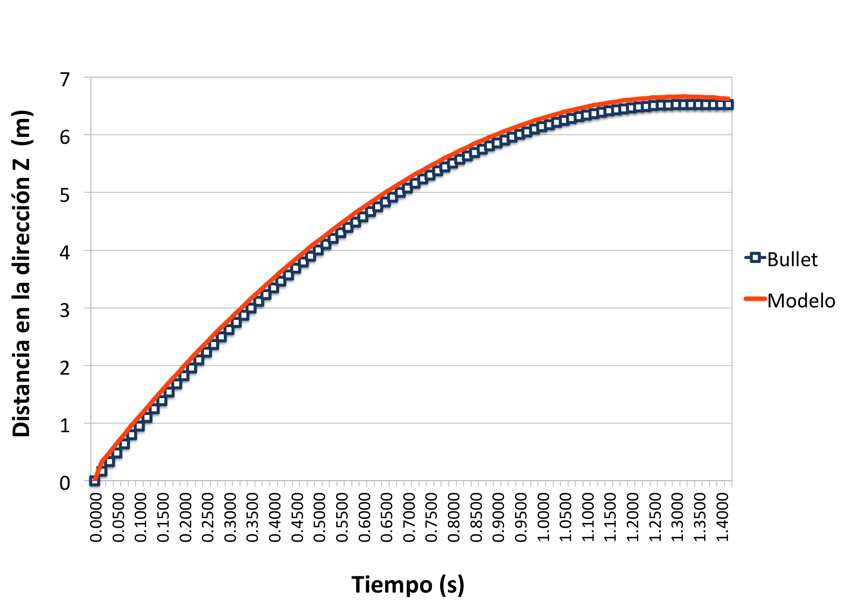
\includegraphics[width=0.75\linewidth]{image002.png} 
    \caption{Con $\mu_d=0.25$} 
    \label{fig1:a} 
    \vspace{4ex}
  \end{subfigure}%% 
  \begin{subfigure}[b]{0.5\linewidth}
    \centering
    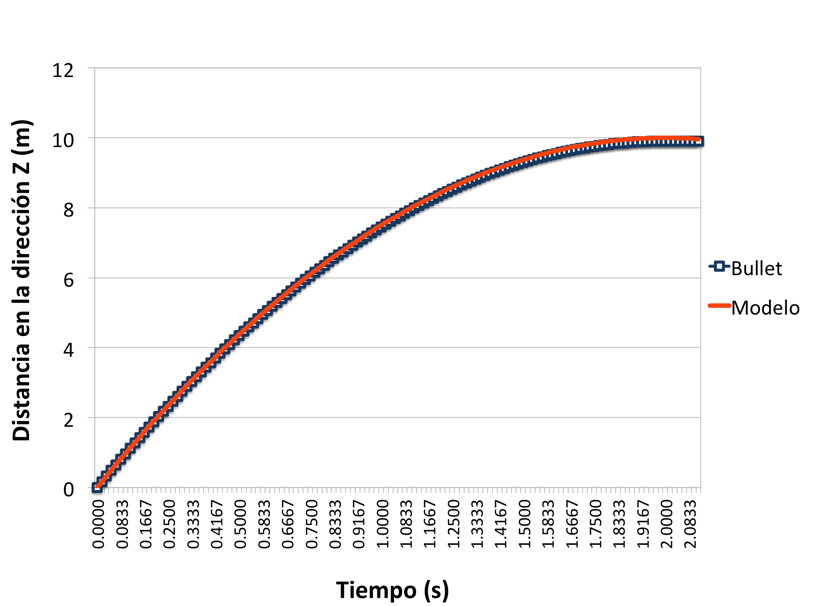
\includegraphics[width=0.75\linewidth]{image003.png} 
    \caption{Con $\mu_d=0.50$} 
    \label{fig1:b} 
    \vspace{4ex}
  \end{subfigure} 
  \begin{subfigure}[b]{\linewidth}
    \centering
    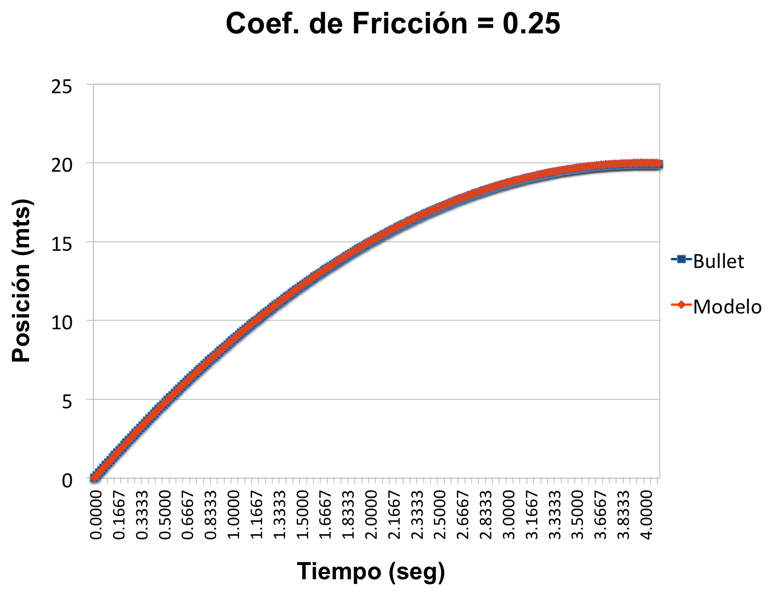
\includegraphics[width=0.4\linewidth]{image001.png} 
    \caption{Con $\mu_d=0.75$} 
    \label{fig1:c} 
  \end{subfigure}%%
  \caption{Experimentos con $v_i = 10$ m/s}
  \label{fig1} 
  \vspace*{4ex}
\end{figure}

\begin{figure}[ht] 
  \begin{subfigure}[b]{0.5\linewidth}
    \centering
    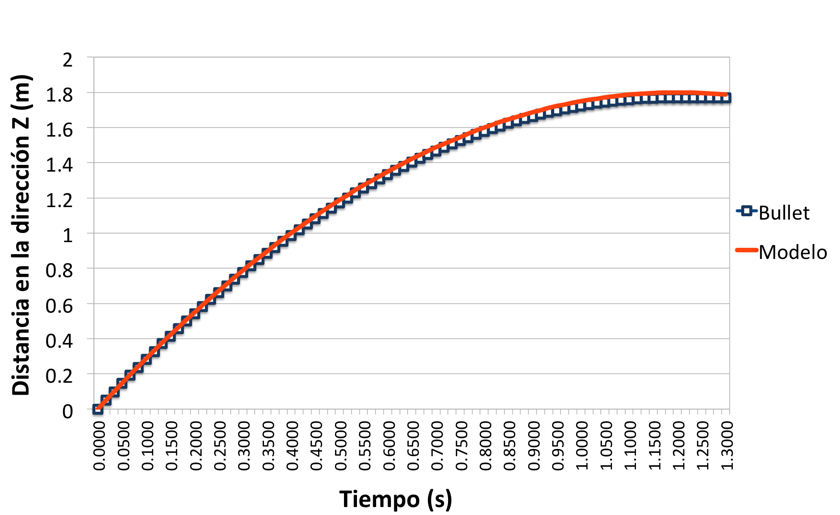
\includegraphics[width=0.75\linewidth]{image009.png} 
    \caption{Con $\mu_d=0.25$} 
    \label{fig2:a} 
    \vspace{4ex}
  \end{subfigure}%% 
  \begin{subfigure}[b]{0.5\linewidth}
    \centering
    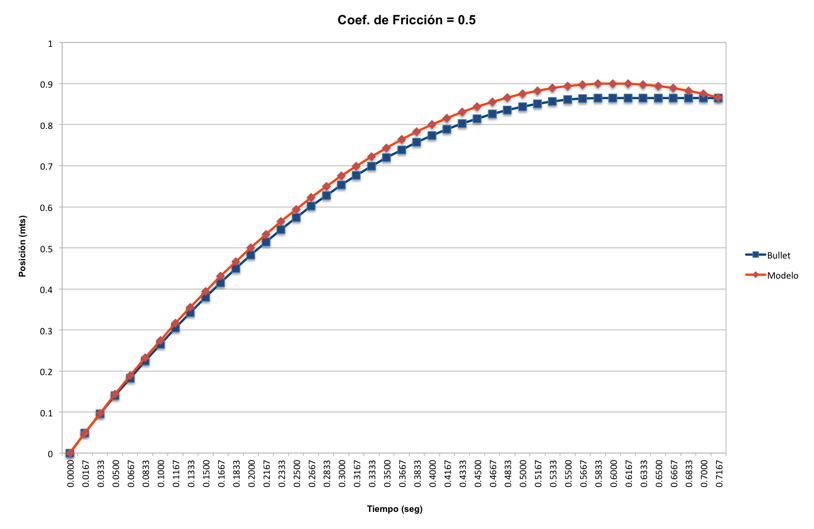
\includegraphics[width=0.75\linewidth]{image007.png} 
    \caption{Con $\mu_d=0.50$} 
    \label{fig2:b} 
    \vspace{4ex}
  \end{subfigure} 
  \begin{subfigure}[b]{\linewidth}
    \centering
    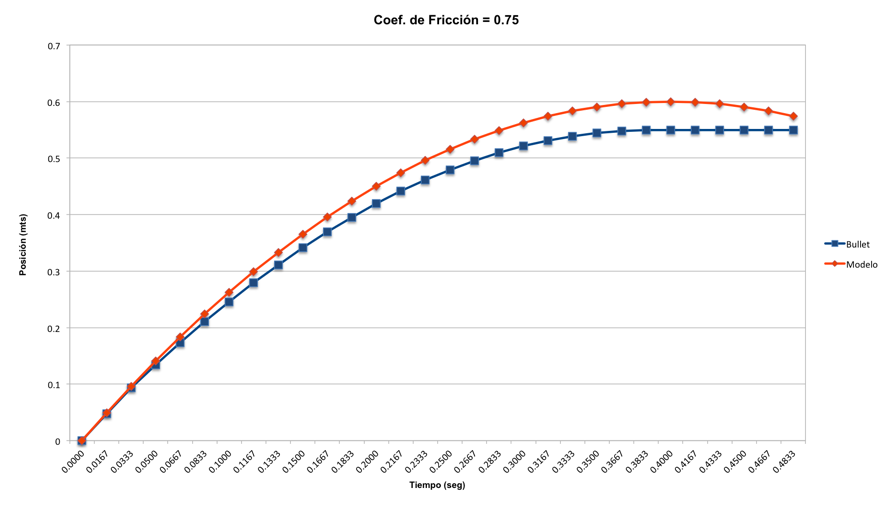
\includegraphics[width=0.4\linewidth]{image008.png} 
    \caption{Con $\mu_d=0.75$} 
    \label{fig2:c} 
  \end{subfigure}%%
  \caption{Experimentos con $v_i = 3$ m/s}
  \label{fig2} 
  \vspace*{4ex}
\end{figure}

\begin{figure}[!ht] 
  \begin{subfigure}[b]{0.5\linewidth}
    \centering
    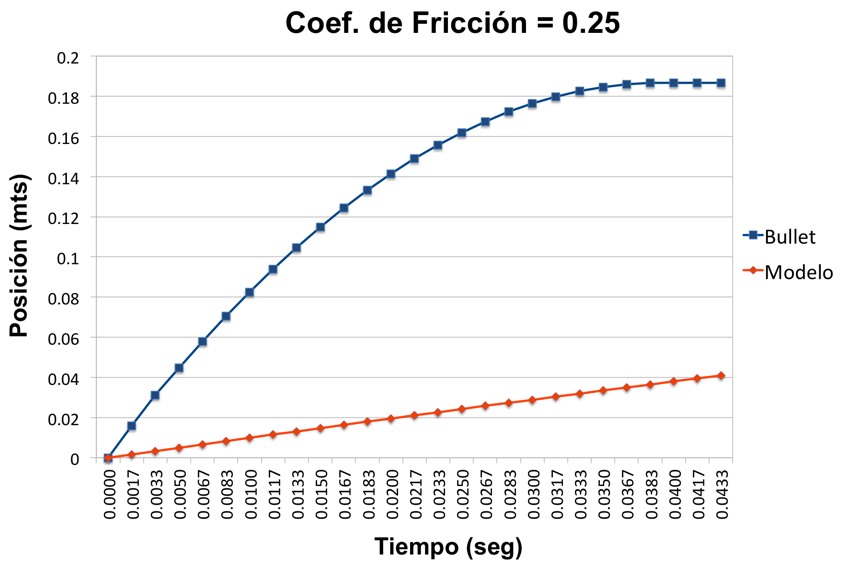
\includegraphics[width=0.75\linewidth]{image004.png} 
    \caption{Con $\mu_d=0.25$} 
    \label{fig3:a} 
    \vspace{4ex}
  \end{subfigure}%% 
  \begin{subfigure}[b]{0.5\linewidth}
    \centering
    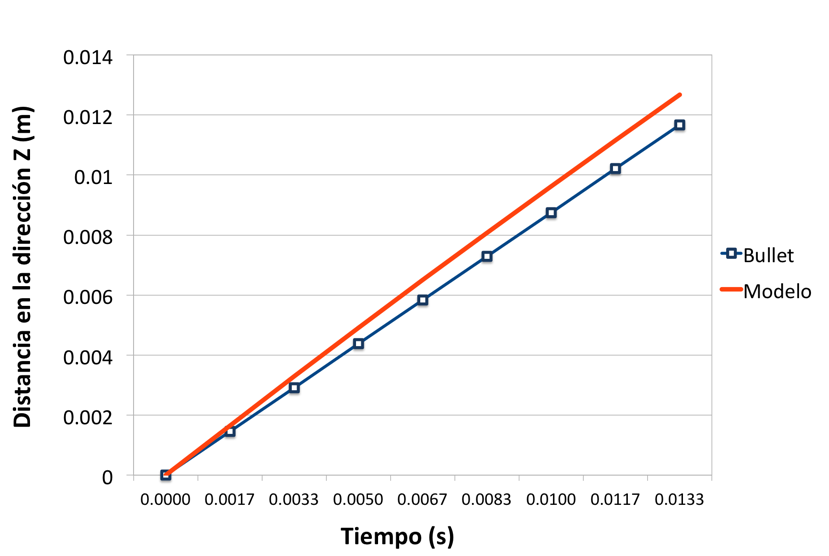
\includegraphics[width=0.75\linewidth]{image005.png} 
    \caption{Con $\mu_d=0.50$} 
    \label{fig3:b} 
    \vspace{4ex}
  \end{subfigure} 
  \begin{subfigure}[b]{\linewidth}
    \centering
    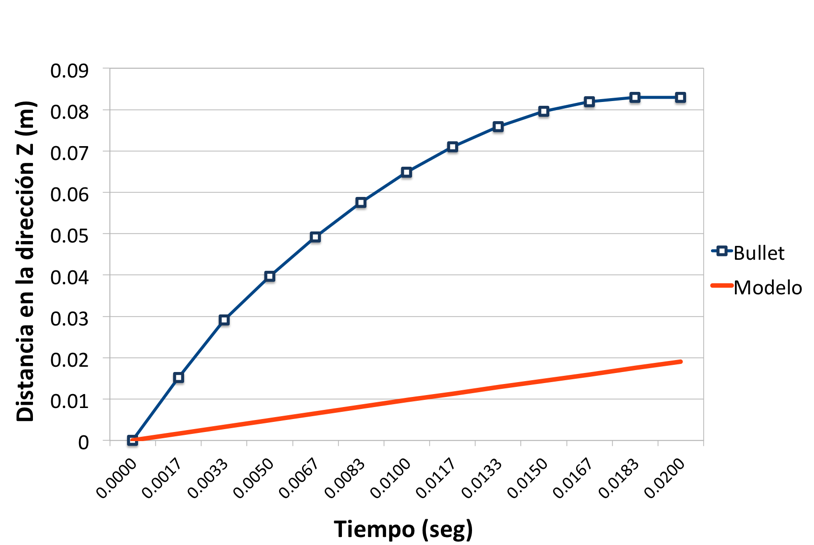
\includegraphics[width=0.4\linewidth]{image006.png} 
    \caption{Con $\mu_d=0.75$} 
    \label{fig3:c} 
  \end{subfigure}%%
  \caption{Experimentos con $v_i = 1$ m/s}
  \label{fig3} 
\end{figure}


\item El segundo simula una esfera a una altura determinada sobre el suelo, que tiene una rapidez constante en el eje perpendicular al piso y que eventualmente colisiona contra el mismo. Se desea comprobar que la colisi\'on entre el cuerpo y el suelo respete el modelo de colisiones el\'asticas y que la velocidad final de la esfera despu\'es del choque sea proporcional al coeficiente de restituci\'on de la misma.\\ 
 \begin{equation}
  e = \frac{v_f}{v_i}
\end{equation}
\\Los resultados exponen una limitaci\'on del motor f\'isico: no representa correctamente las colisiones el\'asticas entre esferas y cuerpos r\'igidos, que ocurren a velocidades bajas. Esto queda en evidencia en los experimentos 1,2,3 y 4. En cada uno de ellos el error fue de casi el 100\%.\\
La raz\'on por la que ocurre este hecho se debe a que Bullet utiliza un algoritmo de colisi\'on que frena la velocidad de un objeto que est\'a a punto de colisionar, haciendo esto puede evitar que los s\'olidos se traspasen y de esta forma se pueden realizar c\'alculos de fuerza m\'as precisos. En el caso de los experimentos, las esferas poseen una rapidez muy baja, cuando est\'an a punto de colisionar Bullet reduce a\'un m\'as esta velocidad y eventualmente quedan con una velocidad tan baja que al chocar contra el suelo se aplica el efecto restitutivo a esta rapidez casi nula y se resuelve que la esfera debe queda en reposo, cuando en realidad deber\'ia poseer una velocidad baja, pero no despreciable. \\

\end{itemize}


%\end{adjustwidth}

\subsubsection{Ventajas}
%\begin{adjustwidth}{1.3cm}{0cm}
\begin{itemize}[leftmargin=5.5mm]
\item C\'odigo abierto: mayor conocimiento sobre las f\'ormulas y m\'etodos implementados en el motor, a diferencia de lo acaecido en trabajos previos \cite{Cuadrupedo}, en donde al usar frameworks f\'isicos de c\'odigo cerrado, no se ten\'ia ni control ni conocimiento pleno de su funcionamiento.
\item Soporte de la comunidad cientf\'ifica.
\item Licencia libre.

\end{itemize}
%\end{adjustwidth}

\subsubsection{Desventajas}
%\begin{adjustwidth}{1.3cm}{0cm}
\begin{itemize}[leftmargin=5.5mm]
\item Documentaci\'on poco clara y desordenada.
\item Implementado en C++: al no formar este lenguaje parte de la expertise del equipo, fue m\'as dif\'icil de desarrollar.
\end{itemize}
%\end{adjustwidth}




\subsection{Librer\'ia de Algoritmos Gen\'eticos}

%\begin{adjustwidth}{1.2cm}{0cm}
Se utiliz\'o la conocida librer\'ia de Algoritmos Gen\'eticos para C++ GaLib, desarrollada por Matthew Wall del MIT \cite{LinkGaLib}.  Ofrece funcionalidades como: programaci\'on paralela, diversos m\'etodos de selecci\'on (elite, ruleta), estrategias de reemplazo (de padres, aleatorio, del peor), entre otras.\\
Se podr\'ia haber implementado una librer\'ia propia; pero hubo que desestimarla, considerando el tiempo requerido y su complejidad.

%\end{adjustwidth}

\subsection{C\'odigo Fuente}

%\begin{adjustwidth}{1.2cm}{0cm}
Al estar Bullet implementado en C++, el c\'odigo fuente tambi\'en est\'a desarrollado en ese lenguaje. En Bullet, se define un World -o mundo f\'isico- en donde se puede insertar, entre otras cosas, cuerpos r\'igidos. En este caso en particular, el mundo consta de un plano  -el suelo- y  el humanoide encima -compuesto por cuerpos r\'igidos y otros elementos f\'isicos-. \\
El programa incluye tanto la visualizaci\'on gr\'afica de la simulaci\'on f\'isica de Bullet del humanoide, as\'i como el algoritmo gen\'etico -y la definic\'on de los individuos, fitness, etc. y su integraci\'on con GaLib-.
\\El c\'odigo fuente se adjunta a esta presentaci\'on y una descripci\'on del mismo y modo de uso e instalaci\'on en el manual de usuario.

%\end{adjustwidth}

%\end{adjustwidth}



\section{Modelo Utilizado}

%\begin{adjustwidth}{1.1cm}{0cm}
Hay diversos modelos. Algunos son m\'as gen\'ericos \cite{flexibleMuscle} \cite{Wojtyra} y complejos.  Sin embargo, se procur\'o utilizar uno que fuera sencillo pero representativo a la vez.\\ 
Se modela al cuerpo humano, con el motor Bullet Physics, como un conjunto de segmentos unidos por articulaciones. A cada uno de ellos se les aplica una fuerza en el centro de masa de cada segmento (denominada Actuador). Que la caminata se produzca o no, depende del tipo de actuador utilizado (la funci\'on utilizada para la fuerza), y de sus par\'ametros. El objetivo, entonces, se reduce a encontrar dichos par\'ametros. Para eso se usan los algoritmos gen\'eticos, un m\'etodo de Inteligencia Artificial. De este modo, se obtiene, de forma an\'aloga a la selecci\'on natural, los individuos que mejor se adapten a la caminata. Tanto los actuadores como el algoritmo gen\'etico se explicar\'an m\'as adelante. \\ 

\subsection{Composici\'on F\'isica del Humanoide}
Como ya se dijo, el humanoide fue modelado en Bullet como un conjunto de segmentos, unidos por articulaciones. Los segmentos son cuerpos rig\'idos 

Se dividi\'o al cuerpo humano en los siguientes segmentos: cabeza, tronco, miembro superior, pelvis y miembro inferior (muslo, pierna y pie). Considerar la mitad superior del cuerpo implicaba tener    Para la simplificaci\'on del problema \\ \\
A continuaci\'on se presenta la composici\'on de cada segmento (de acuerdo a la biomec\'anica) 
\begin {table}[ht]
	\begin{center}
		\begin{tabular}{ | c | c | c | c | c | c |}
	  		 \hline
	  		Parte & Cantidad & Forma & Largo (en m) & Peso (en kg) & Uniones\\
	  		\hline 
	  		\hline
	  		Pelvis & 1 & esf\'erico & 0.08655 & 9.9718 & Cadera\\
	  		\hline
	  		Muslo & 2 & esfero-cilindro & 0.4015 & 10.3368 & Cadera y Rodilla\\
	  		\hline
	  		Pierna & 2 & esfero-cilindro &  0.4015 & 3.1609 & Rodilla y Tobillo\\
	  		\hline
	  		Pie & 2 & esfero-cilindro & - & 1.0001 & Tobillo\\
	  		\hline
		\end{tabular}
		\caption{Segmentos del humanoide}
	\end{center}
\end{table}
%\end{adjustwidth}

\subsection{Articulaciones}
Para unir los distintos segmentos entre s\'i, se utilizaron articulaciones bisagra con 2 grados de libertad: en el eje Z -en donde ocurre la caminata- y en el eje Y -el perpendicular al piso-. Adem\'as, para cada caso en particular, se definieron cotas para los \'angulos que pueden existir entre los segmentos. Esto es muy importante, no s\'olo porque se adec\'ua a datos biol\'ogicos, sino porque, de otro modo la caminata no podr\'ia lograrse: si los \'angulos son demasiado altos, la caminata se produce girando las piernas por encima de la pelvis; si por el contrario, son demasiado bajos, las piernas van a estar muy r\'igidas, originando pocos pasos y muy cortos. 
Tanto para la  \\
Por otra parte, a la pelvis se le restringe todo tipo de rotaci\'on. 

\section{Actuadores}
%\begin{adjustwidth}{1.1cm}{0cm}

Para representar la fuerza aplicada a cada uno de los segmentos, se utilizaron diferentes funciones (todas ellas peri\'odicas). A fin de simplificar el modelo, el humanoide tiene el mismo tipo de actuador aplicado en todos los segmentos.

\subsection{Gen\'erico}

\begin{equation}
  f(t) =  A_1 \sin(\omega_1t+\phi)+A_2 \cos(\omega_2t+\phi)+C
\end{equation}

\subsection{Fourier}

\begin{equation}
  f(t) =  A_1 \sin(\omega t+\phi)+B_1 \cos(\omega t+\phi)+A_2 \sin(2\omega t+\phi)+B_2 \cos(2\omega t+\phi)+C
\end{equation}

\subsection{Extra Fourier}

\begin{equation}
\begin{split}
  f(t) = &   A_1 \sin(\omega t+\phi)+B_1 \cos(\omega t+\phi)+A_2 \sin(2\omega t+\phi)+B_2 \cos(2\omega t+\phi) \\
  &+A_3 \sin(3\omega t+\phi)+B_3 \cos(3\omega t+\phi)+A_4 \sin(4\omega t+\phi)+B_4 \cos(4\omega t+\phi) \\ 
  &+A_5 \sin(5\omega t+\phi)+B_5 \cos(5\omega t+\phi)+A_6 \sin(6\omega t+\phi)+B_6 \cos(6\omega t+\phi) \\
  &+A_7 \sin(7\omega t+\phi)+B_7 \cos(7\omega t+\phi)+A_8 \sin(8\omega t+\phi)+B_8 \cos(8\omega t+\phi) \\
  &+A_9 \sin(9\omega t+\phi)+B_9 \cos(9\omega t+\phi) + C
\end{split}
\end{equation}

\subsection{Doble coseno}

\begin{equation}
\begin{aligned}[c]
\psi (t) = t+ \phi- \floor[\Bigg]{ \frac{t+\phi}{\pi/\omega_1+\pi/\omega_2} } (\pi/\omega_1+\pi/\omega_2) 
 \end{aligned}
 \qquad
 \begin{aligned}[c]
 \psi: \mathbb{Re} \rightarrow \bigg[0, \frac{2\pi}{\omega}\bigg] 
 \end{aligned}
 \end{equation}
 \\
\begin{equation}
\omega = \frac{2\omega_1 \omega_2}{\omega_1+\omega_2} 
 \end{equation}
\\
\begin{equation}
f(t) =  \left\{
\begin{array}{ll}
      A \cos(\omega_1 \psi(t))+C & \mbox{si $\omega_1 \psi(t) < \pi$}  \\
      A \cos(\omega_2 (\psi(t) - (\pi/\omega_1) + (\pi/\omega_2 ) ) )+C & \mbox{en otro caso$$} \\
\end{array} 
\right. 
 \end{equation}

\section{Funci\'on de Partida}

%\begin{adjustwidth}{1.1cm}{0cm}
xxxxx
%\end{adjustwidth}


%----------------------------------------------------------------------------------------
%	SECTION 2
%----------------------------------------------------------------------------------------

\section{Algoritmo Gen\'etico}


\subsection{Individuo}

%\begin{adjustwidth}{1.25cm}{0cm}
Para simplificar 
%\end{adjustwidth}

\subsection{Fitness}

%\begin{adjustwidth}{1.25cm}{0cm}
El papel de la funci\'on de fitness en un algoritmo gen\'etico es evaluar qu\'e tan bueno es un individuo. En este caso, est\'a definida como un producto de tres m\'odulos o propiedades: altura, velocidad y direcci\'on:
\begin{equation}
  fitness = altura * velocidad * direcci\acute{o}n
\end{equation}
Los tres tienen la misma importancia y, por eso, como se ver\'a a continuaci\'on, est\'an definidos de forma similar (con una funci\'on exponencial y pueden valer entre 0 y 1). Con todo esto, dado que el fitness est\'a pensado como un producto, basta con que uno de los m\'odulos sea muy chico para  ``anular'' al individuo -es decir, otorgarle un valor que tiende a cero-. Sin embargo, los diferentes m\'odulos no son completamente independientes entre s\'i: por ejemplo, si la altura es demasiado baja, posiblemente la velocidad y la direcci\'on no sean adecuadas. \\
%\end{adjustwidth}

\subsubsection{Altura}
\label{altura}
%\begin{adjustwidth}{1.4cm}{0cm}
Es un factor relacionado con la altura del individuo en toda la simulaci\'on, y se expresa:\\
\begin{equation}
  altura = \frac{\sum_{n=0}^{T} {e^{-C( h_{t_{n}} - h_{t_{0}} )^2  }}}{simulation\_steps}
\end{equation}
\\ donde $t_{0}$ es el tiempo inicial, $t_{T}$ el tiempo final, simulation\_steps la cantidad pasos de simulaci\'on y C una constante adimensional que vale 5 (dato experimental).
\\
Se calcula a partir de la diferencia entre la altura en cada instante de la simulaci\'on, con su altura inicial -la altura est\'a definida como la posici\'on de la pelvis en el eje Z-. Cuanto mayor sea esa diferencia, m\'as r\'apido el individuo cae, y por eso este m\'odulo tiende a cero. Por el contrario, valdr\'a uno si la diferencia es \'infima -lo que significa que el humanoide mantiene su misma altura durante la caminata-.\\

%\end{adjustwidth}

\subsubsection{Velocidad}
\label{velocidad}
%\begin{adjustwidth}{1.4cm}{0cm}
Indica qu\'e tan cercana es la velocidad del individuo con respecto a una velocidad objetivo -en este caso, es de 1.2 m/h-, y se expresa de la siguiente forma:\\
\begin{equation}
  velocidad = \frac{\sum_{n=0}^{T} {e^{-C( \|v_{t_{n}}\| - V_{O} )^2  }}}{simulation\_steps}
\end{equation}
\\ donde $t_{0}$ es el tiempo inicial, $t_{T}$ el tiempo final, $V_{O}$ la velocidad objetivo en el eje Z -el eje de la caminata-, simulation\_steps la cantidad pasos de simulaci\'on y C es una constante adimensional que vale 5 (dato experimental).
\\
Sigue una l\'ogica y c\'alculo similares al factor de altura: a mayor discrepancia de la velocidad real del humanoide con $V_{O}$, menor -y m\'as cercano a cero- es el valor arrojado por el m\'odulo de velocidad. 

%\end{adjustwidth}

\subsubsection{Direcci\'on}
\label{direccion}
%\begin{adjustwidth}{1.4cm}{0cm}
Se\~nala qu\'e tan similares son la direcci\'on objetivo -un vector unitario, que en este caso se encuentra en el eje Z- y la direcci\'on con la que camine el humanoide. Se calcula como sigue:\\
\begin{equation}
 direcci\acute{o}n = \frac{\sum_{n=0}^{T} {e^{-C( \vec{v_{t_{n}}} \cdot \vec{V_{O} } -1)^2 } } }{simulation\_steps}
\end{equation}
\\ donde $t_{0}$ es el tiempo inicial, $t_{T}$ el tiempo final, $\vec{v_{t_{n}}}$ el versor de la direcci\'on del humanoide en el momento $t_{n}$, $\vec{V_{O}}$ el versor de la direcci\'on objetivo, simulation\_steps la cantidad pasos de simulaci\'on y C es una constante adimensional que vale 5 (dato experimental).
\\ El producto escalar entre los versores responde a la Similitud Coseno: $\cos \theta = \frac{A \cdot B} {\|A\|\|B\| } $, donde A y B son vectores que no se encuentran normalizados, y $\theta$ es el \'angulo formado entre ellos. As\'i,  si $\cos \theta=1$, significa que los vectores est\'an paralelos entre s\'i -que es el efecto buscado en el caso de la direcci\'on-. 
\\ Al producto escalar se le resta 1, para que el m\'odulo sea consistente con la funci\'on exponencial utilizada y que valga 1 cuando $\theta = 0$, y  0 cuando $\theta = \pi$. Cabe aclarar que se trata al \'angulo en forma sim\'etrica, ya que, por ejemplo $\cos(-\pi/6) = \cos(\pi/6)$.

%\end{adjustwidth}



%----------------------------------------------------------------------------------------
%	SECTION 3
%----------------------------------------------------------------------------------------

\subsection{Par\'ametros del Algoritmo}

\subsubsection{M\'etodos de selecci\'on}
\label{metodos de seleccion}
%\begin{adjustwidth}{1.4cm}{0cm}
Varios son los m\'etodos de selecci\'on que son usados con frecuencia: Elite (priorizan en cada generaci\'on los individuos con mejor fitness), y los estoc\'asticos (los individuos que sobreviven en cada generaci\'on  son elegidos probabil\'isticamente), como Rouleta, por Torneos, Boltzmann. \\
Actualmente, la funci\'on de fitness involucra caracter\'isticas muy restrictivas (como la simetr\'ia y el hecho de prohibir que los pies est\'en por encima de la pelvis). Utilizar m\'etodos de selecci\'on que prioricen lo estoc\'astico no resulta conveniente (pues mayor ser\'a la probabilidad de generar individuos no favorables). Por eso, se utiliz\'o un m\'etodo un poco m\'as elitista, como el de Torneos. La probabilidad es de 0.7.
%\end{adjustwidth}

\subsubsection{M\'etodos de cruza}
\label{metodos de cruza}
%\begin{adjustwidth}{1.4cm}{0cm}
xxxx
%\end{adjustwidth}

\subsubsection{Mutaci\'on}
\label{mutacion}
%\begin{adjustwidth}{1.4cm}{0cm}
xxxx
%\end{adjustwidth}



%----------------------------------------------------------------------------------------
%	SECTION 4
%----------------------------------------------------------------------------------------

\section{Resultados Obtenidos}
%\begin{adjustwidth}{1.1cm}{0cm}
cccccccvvvvv

\begin{figure}[h]
\begin{center}

\includegraphics[width=0.65\textwidth]{placeholder} % Include the image placeholder.png
\caption{Figure caption.}
\end{center}
\end{figure}
%\end{adjustwidth}

%----------------------------------------------------------------------------------------
%	SECTION 5
%----------------------------------------------------------------------------------------

\section{Conclusiones}

%\begin{adjustwidth}{1.1cm}{0cm}
xxxxxxxx
%\end{adjustwidth}

%----------------------------------------------------------------------------------------
%	BIBLIOGRAPHY
%----------------------------------------------------------------------------------------

\begin{thebibliography}{1}
\bibitem{Libro1}
John Mattews and Kurtis Fink, \emph{M\'etodos Num\'ericos con Matlab, Fecha de publicacion: Mayo 2000 | ISBN-10: 8483221810 | ISBN-13: 978-8483221815 | Edicion: 3}
\bibitem{LinkBullet} Sitio web de Bullet Physics: http://www.bulletphysics.org/
\bibitem{Cuadrupedo}
Kevin Kenny, M\'aximo Videla y Axel Wassington, \emph{Simulaci\'on y Animaci\'on Biomec\'anica de un Cuadr\'upedo, 2014 | ITBA}
\bibitem{Comparissons}
Andreas Gerndt y otros, \emph{An Evaluation of Open Source Physics Engines for Use in Virtual Reality Assembly Simulations, Fecha de publicaci\'on: 2012}
\bibitem{LinkGaLib} Sitio web de GaLib: http://lancet.mit.edu/ga/
\bibitem{flexibleMuscle}
Thomas Geijtenbeek, Michiel van de Panne y A. Frank van der Stappen, \emph{Flexible Muscle-Based Locomotion for Bipedal Creatures, 2013 }
\bibitem{Wojtyra}
Marek Wojtyra, \emph{Multibody Simulation Model of Human Walking, 2003 | Warsaw University of Technology}
\bibitem{biomechanics} http://www.exrx.net/Kinesiology/Segments.html
\end{thebibliography}

%----------------------------------------------------------------------------------------


\end{document}